
%(BEGIN_QUESTION)
% Copyright 2010, Tony R. Kuphaldt, released under the Creative Commons Attribution License (v 1.0)
% This means you may do almost anything with this work of mine, so long as you give me proper credit

Skisser tilkoblingsledninger som viser hvordan du kan simulere et {\it termoelement}-signal inn på denne elektroniske temperaturtransmitteren ved hjelp av et potensiometer og et batteri:

$$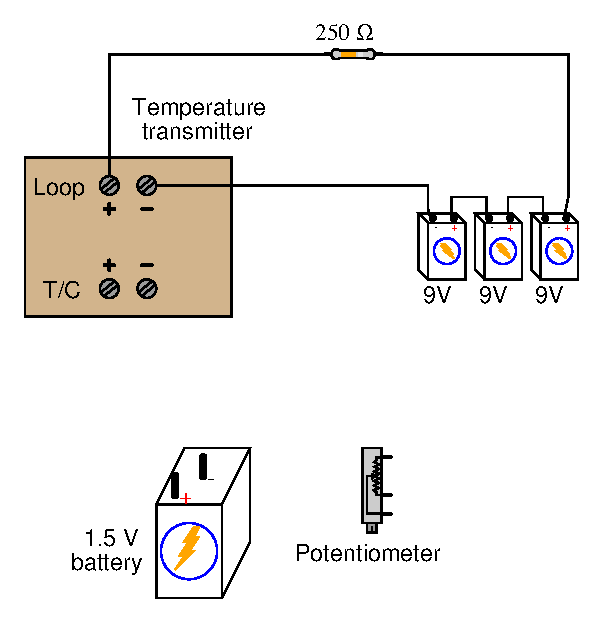
\includegraphics[width=15.5cm]{i00591x01.eps}$$

Anta at transmitteren er riktig konfigurert for termoelementinngang, og at potensiometeret har tilstrekkelig presisjon og oppløsning slik at det ikke er nødvendig å koble det med andre motstander i et nettverk.

\underbar{file i00591}
%(END_QUESTION)





%(BEGIN_ANSWER)

$$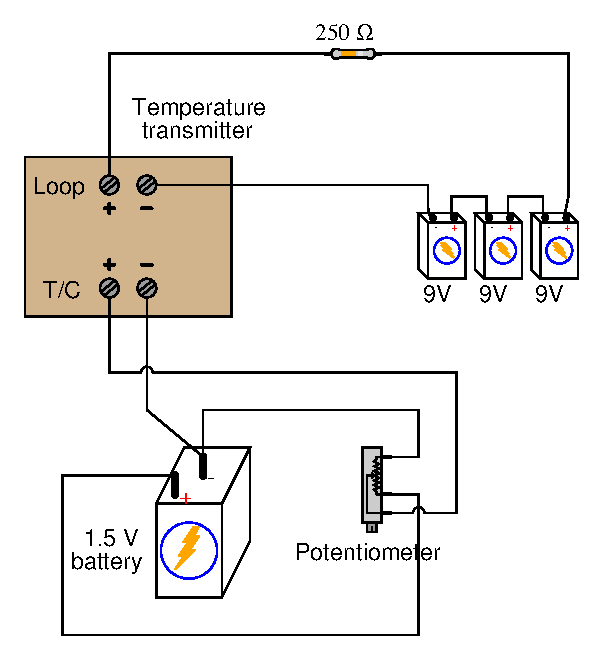
\includegraphics[width=15.5cm]{i00591x02.eps}$$

Enhver korrekt løsning vil inneholde disse egenskapene:

\begin{itemize}
\item{} 1.5 V batteri koblet over hele potensiometerspennet
\item{} Viskerterminal koblet til én inngangsterminal på transmitteren
\item{} Den andre inngangsterminalen på transmitteren koblet til riktig pol på batteriet (polariteter må stemme)
\end{itemize}

%(END_ANSWER)





%(BEGIN_NOTES)

{\bf Dette spørsmålet er ment for eksamen og ikke arbeidsark!}.

%(END_NOTES)

